\section{Generative Modeling 1}

\begin{figure}[!h]
    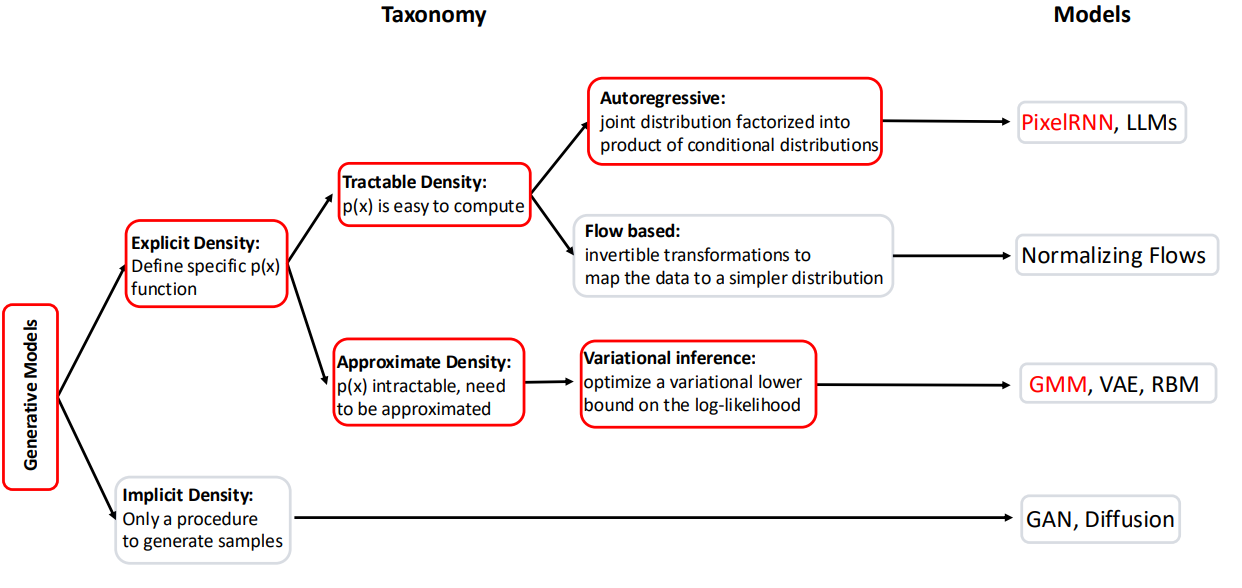
\includegraphics[width = \columnwidth]{figures/GenAI1/GenAIOverview.png}
\end{figure}
\textbf{Goal}: \(p_{data} \sim p_{model}\)

Model the data's density distribution.
If accurate, we can sample  new points from the distribution an they will be properly correlated such that the new instance looks like it came from the data distribution.
\subsection{Overview}
\subsubsection{Probability density function}
\(p(x) \ge 0, \forall_x \in X\) Always positive 

\(\int_X p(x)dx = 1\) Probability must sum to one

Elements in the support compete in a zero sum game for probability mass density.
\subsubsection{Discriminative Model}
Learn probability distribution \(p(y|x)\)

Discriminant models.
The possible labels compete for probability mass but not the images themselves.
\begin{figure}[!h]
    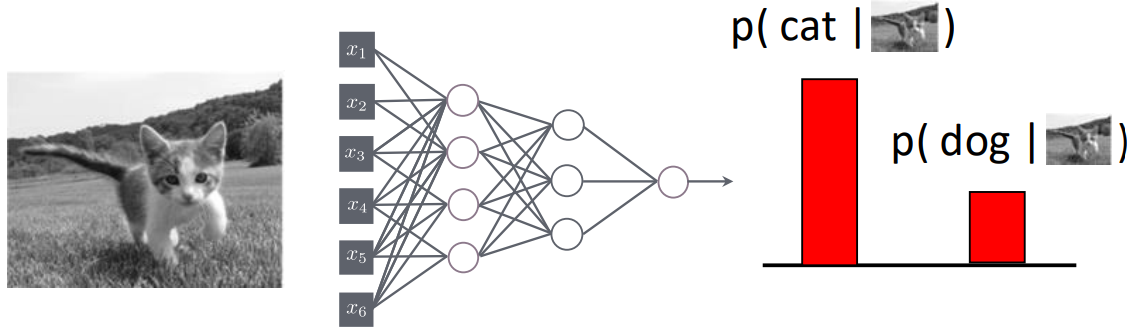
\includegraphics[width = \columnwidth]{figures/GenAI1/DiscriminativeModel.png}
\end{figure}


\subsubsection{Generative Model}
Learn a probability distribution \(p(x)\)

Generative models can reject unreasonable images by assigning them low mass.
\begin{figure}[!h]
    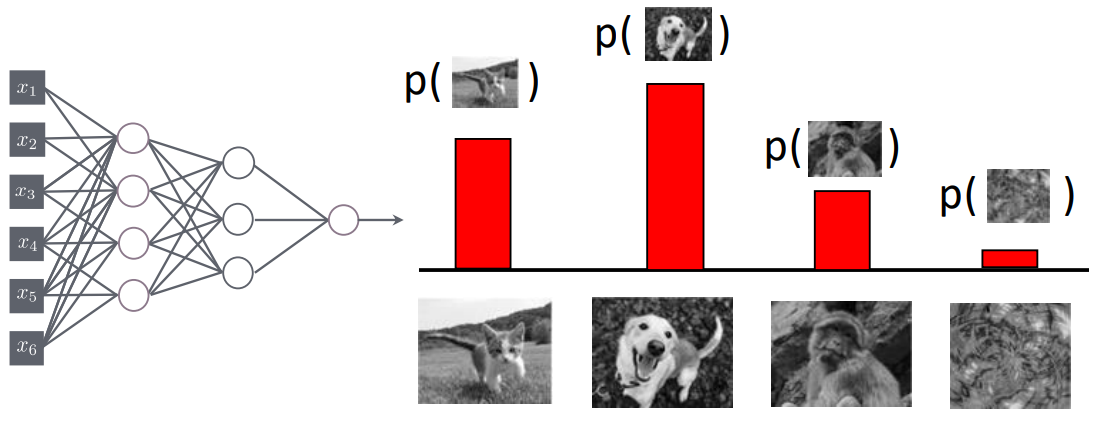
\includegraphics[width = \columnwidth]{figures/GenAI1/GenerativeModel.png}
\end{figure}

Generative models: All possible images compete against one another for probability mass.

Requires deep image understanding, is a dog more likely to sit or stand? How likely is a three legged dog?

\subsubsection{Conditional Generative Model}
Learn a probability distribution \(p(x|y)\)

\begin{figure}[!h]
    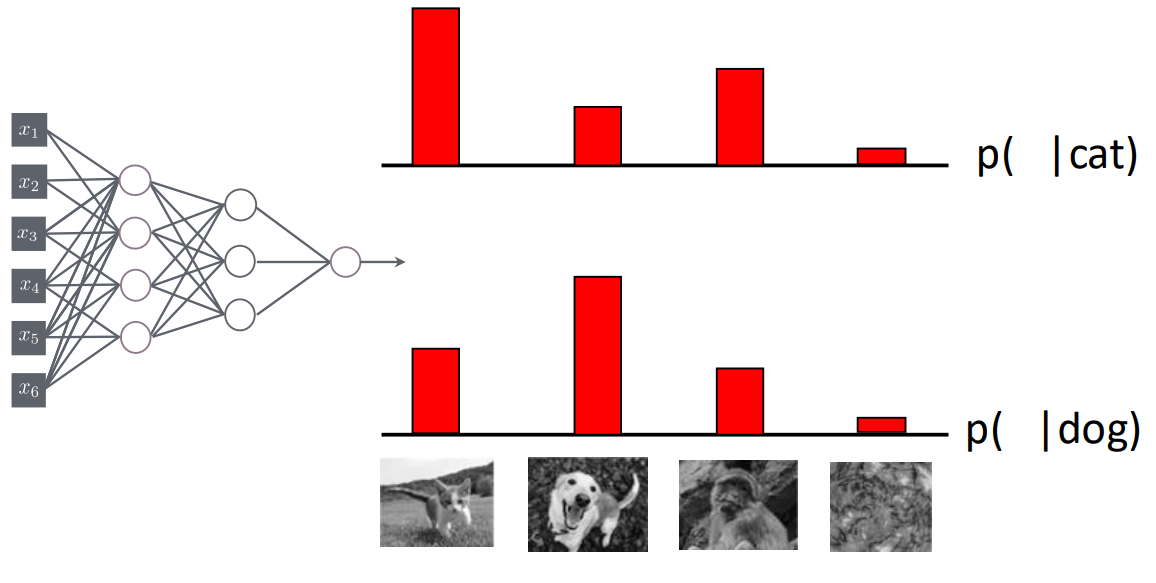
\includegraphics[width = \columnwidth]{figures/GenAI1/ConditionalGenerativeModel.png}
\end{figure}
Conditional Generative models: each label induces a competition amongst all images.

\subsubsection{Bayes formula for Generative Models}
\[
P(x|y) = \frac{P(y|x)}{P(y)}P(x)
\]

\begin{itemize}
    \item \textbf{Conditional generative model} \(P(x|y)\): Probability of the given data a certain class
    \item \textbf{Discriminant model} \(P(y|x)\):Given the data how likely is a label
    \item \textbf{Marginal probability} \(P(y)\):Frequency of occurence
    \item \textbf{Generative model} \(P(x)\): GAN, VAE, etc. 
\end{itemize}

\subsubsection{Shannon Entropy}
\[
H(p) = - \sum_x p(x) \text{log} p(x)
\]
\begin{figure}[!h]
    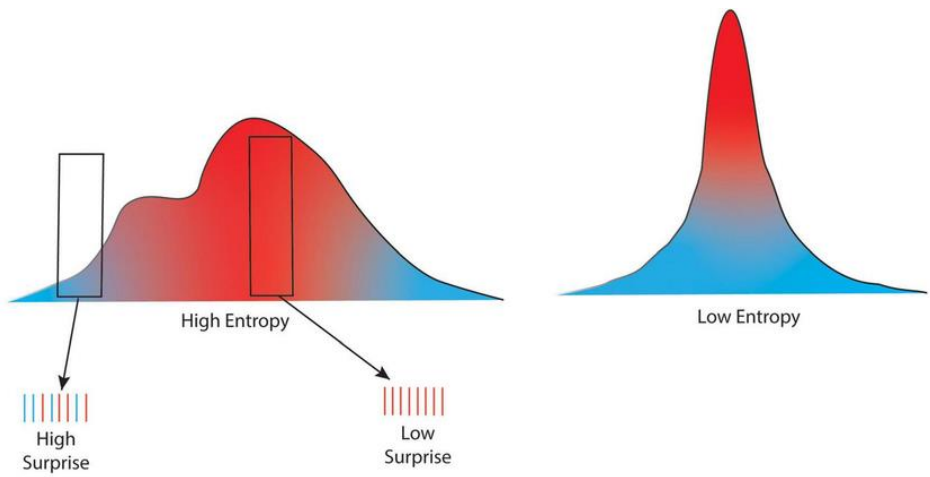
\includegraphics[width = \columnwidth]{figures/GenAI1/ShannonEntropy.png}
\end{figure}

\subsubsection{Cross Entropy}
Commonly used as a loss function for classification tasks.
Measures the additional number of bits of information necessary to determine a random variable when using an estimate \(q\) of the true probability distribution \(p\).

Measure how uncertain we are about the models output value.
Can only be as uncertain as the entropy of the labels.
Always greater then zero.
\[
H(p,q) = - \sum_x p(x) \text{log} q(x) = H(p) + D_{KL}(p||q)
\]
\subsection{Gaussian models}

Goal = accurately model the probability density of the data

It means find the parameters of our model that make the data most probable under the distribution.

\subsubsection*{Likelihood function}
Measures the probability of the observing the given data as a function of the parameters of the chosen statistical model.

\textbf{Dataset}: \(X = \left\{x^{(1)},x^{(2)},\dots,x^{(n)}\right\}\)

\textbf{Family of probability density functions}: \(f_\theta(x)\)

\textbf{Likelihood function}: \(L(\theta) = \prod_{i = 1}^{n}f_\theta(x_i)\)

This is th probability of the data assuming i.i.d under chosen set of parameters

\textbf{Log-likelihood function}: \(l(\theta) = \sum_{i = 1}^{n} \text{log}f_\theta(x_i)\)

Easier to work with and allowed since monotonically increasing function
\begin{itemize}
    \item Numerical stability, prevents underflow (very small numbers)
    \item Easier deriviations
    \item Easier smoother loss landscape for gradient descent
\end{itemize}

\subsubsection*{Maximal likelihood estimate (MLE)}
Estimating the parameters \(\theta\) of a probability distribution/model that maximizes the likelihood of the data \(X\).
\[
\theta_{MLE}^* = \arg\max_{\theta} P(X|\theta) =  \arg\max_{\theta} \sum_{i = 1}^{n} \text{log} f_\theta(x_i)
\]

Note, this does not guarantee that the log likelihood of the data is maximized, only that it is maximized for this particular family of probability distributions. 
It might be that more complex families fir the data better. 

\subsubsection{Problem}
Our model will fail in the simple case where the data follows bimodal distribution.
We need more felxible models that can efficiently estimate the complex distributions that naturally arise from our data.

\subsection{Gaussian mixture models}
Increase the models complexity.

K-Gaussian distributions, each ones shape controlled by the covariance matrix and mean vector.
\begin{figure}[!h]
    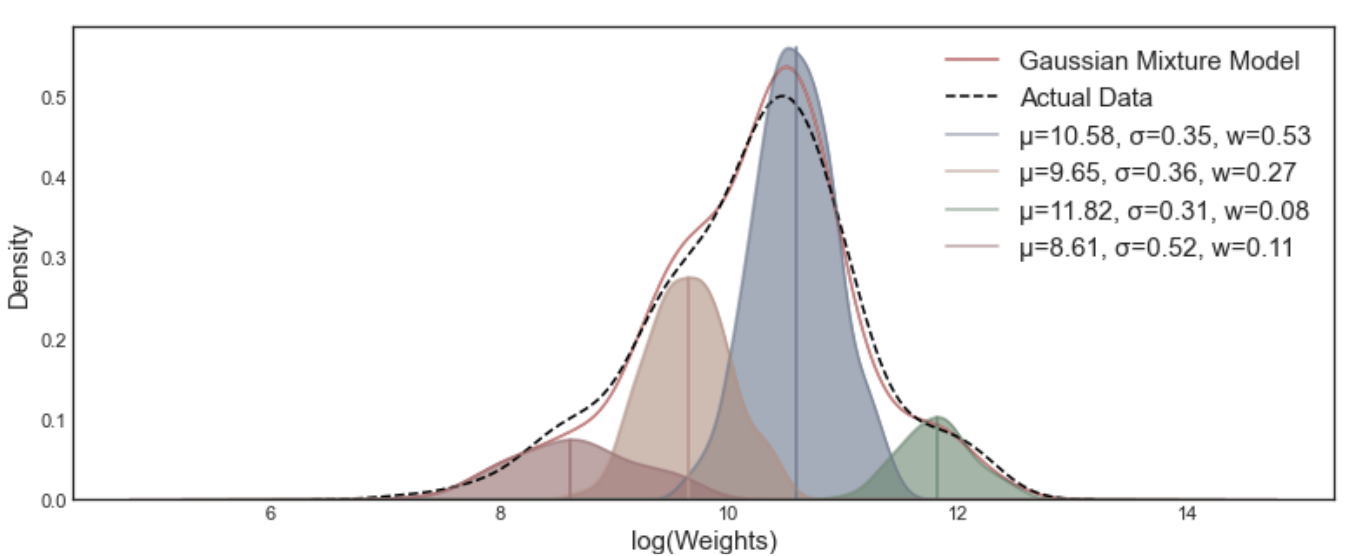
\includegraphics[width = \columnwidth]{figures/GenAI1/GMM.png}
\end{figure}
We need better ways to optimize complex models.
MLE formalism is ill defiend resulting in mode collapse when \(x_n = \mu_j\).

We dont know how many Gaussians we need nor where they are.
We need latent variables.
Latent variables helps explain patterns in data we can observe.
\subsubsection{Expectation Maximization Algorithm}
An algorithm that helps latent variable models locate a local maximum for the likelihood function by iterating over a two step procedure.

\begin{enumerate}
    \item Initiate K random multivariant Guassuan distribution.
    \item E-Step(Freeze parameters and make prior q = posterior): Describe each points probability of being owend by each source. P that of point under k'th Gaussian divided by sum of P for all other Gaussian.
    \item M-step (Freeze q and update parameters to maximize p):Update Gaussian parameters to maximize likelihood using probabilistic center of mass.
    \item Repeat E- and M-step until likelihood falls bellow a set theshold.
\end{enumerate}

\begin{figure}[!h]
    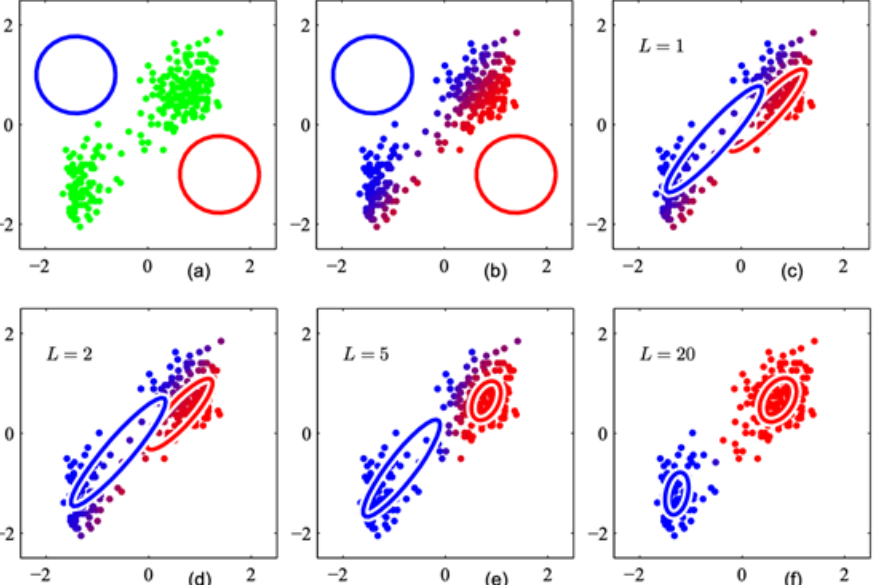
\includegraphics[width = \columnwidth]{figures/GenAI1/EMAlgorithem.png}
\end{figure}